\documentclass{standalone}
\usepackage{tikz,graphics}
\usetikzlibrary{optics, arrows.meta}
\usetikzlibrary{decorations.markings, fpu, decorations.pathreplacing, decorations.text, decorations.footprints, calc}

  
%%%%%%%%%%%%%%	   
\begin{document}
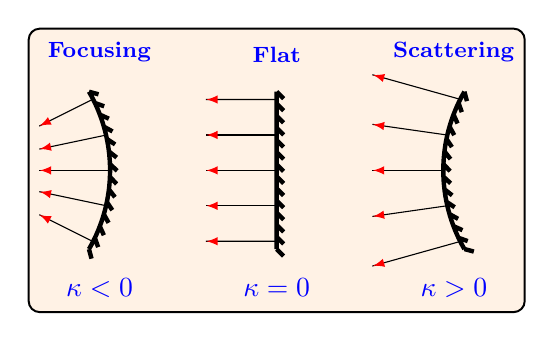
\begin{tikzpicture}[use optics, scale=.45, /pgf/fpu/install only={reciprocal}]
	\draw [line width=0.25mm,rounded corners, fill=orange, fill opacity=0.1](-7,-4) rectangle (7,4);	
	
\node[mirror, black, ultra thick, label={[label distance=0.25cm, blue]north: \footnotesize \textbf{Flat}}, label={[label distance=0.25cm, blue]south: $\kappa =0$}] (S) at (0,0) {};
	\node[spherical mirror, spherical mirror angle=60,  spherical mirror type=concave, black, ultra thick, label={[label distance=0.25cm, blue]north: \footnotesize \textbf{Focusing}}, label={[label distance=0.25cm, blue]south: $\kappa <0$}
	] (M) at (-5,0) {};
\node[spherical mirror, spherical mirror angle=60, spherical mirror type=convex, black, ultra thick, label={[label distance=0.25cm, blue]north: \footnotesize \textbf{Scattering}}, label={[label distance=0.25cm, blue]south: $\kappa >0$}%, draw mirror focus
	] (M) at (5,0) {};
%	\node[spherical mirror, object height=2cm,	spherical mirror angle=3cm, draw mirror focus, draw mirror center={red}] (M) {};
	
\draw[put arrow={at=0.99,arrow=latex,style={red}}]  (0,0) -- (-2cm,0cm);
\draw[put arrow={at=0.99,arrow=latex,style={red}}]  (0,1) -- (-2cm,1cm);
\draw[put arrow={at=0.99,arrow=latex,style={red}}]  (0,2) -- (-2cm,2cm);
\draw[put arrow={at=0.99,arrow=latex,style={red}}]  (0,-1) -- (-2cm,-1cm);
\draw[put arrow={at=0.99,arrow=latex,style={red}}]  (0,-2) -- (-2cm,-2cm);
	
\draw[put arrow={at=0.99,arrow=latex,style={red}}]  (-4.7,0) -- (-6.7cm,0cm);
\draw[put arrow={at=0.99,arrow=latex,style={red}}]  (-4.8,1) -- (-6.7cm,0.6cm);
\draw[put arrow={at=0.99,arrow=latex,style={red}}]  (-5.2,2) -- (-6.7cm,1.25cm);
\draw[put arrow={at=0.99,arrow=latex,style={red}}]  (-4.8,-1) -- (-6.7cm,-0.6cm);
\draw[put arrow={at=0.99,arrow=latex,style={red}}]  (-5.2,-2) -- (-6.7cm,-1.25cm);

	
	\draw[put arrow={at=0.99,arrow=latex,style={red}}]  (4.7,0) -- (2.7cm,0cm);
	\draw[put arrow={at=0.99,arrow=latex,style={red}}]  (4.8,1) -- (2.7cm,1.3cm);
	\draw[put arrow={at=0.99,arrow=latex,style={red}}]  (4.8,-1) -- (2.7cm,-1.3cm);
	\draw[put arrow={at=0.99,arrow=latex,style={red}}]  (5.2,2) -- (2.7cm,2.7cm);
	\draw[put arrow={at=0.99,arrow=latex,style={red}}]  (5.2,-2) -- (2.7cm,-2.7cm);
	

\end{tikzpicture}

\end{document}